\documentclass[11pt]{article}
\input{\string~/.preamble}
\begin{document}


% arg1=pdfurl arg2=pagenum arg3=sectiontitle
% \newcommand{\linksection}[3][../../bishop_pattern_recognition_and_machine_learning.pdf]{
%     \subsection*{\href[page=#2]{#1}{#3}}
% }


\newcommand{\linksection}[3][../bishop_pattern_recognition_and_machine_learning.pdf]{
    \subsection*{\href[page=#2]{#1}{#3}}
}

\newcommand{\linkinline}[3][../../bishop_pattern_recognition_and_machine_learning.pdf]{
    \noindent\href[page=#2]{#1}{#3}
}

\renewcommand{\norm}[1]{\left\lVert#1\right\rVert}
\renewcommand{\E}[2][]{\mathbb{E}_{#1}\left\{#2\right\}}
\newcommand{\var}[2][]{var_{#1}\left\{#2\right\}}
\newcommand{\cov}[1]{cov\{#1\}} 
\newcommand{\normal}[1]{\mathcal{N}\left(#1\right)}
\newcommand{\exponents}[1]{exp\left\{#1\right\}}
\newcommand{\kl}[2]{\textbf{KL}\left(#1 || #2\right)}


\newcommand{\bmu}{\boldsymbol{\mu}}
\newcommand{\bpi}{\boldsymbol{\pi}}
\newcommand{\bTheta}{\boldsymbol{\Theta}}
\newcommand{\bSigma}{\boldsymbol{\Sigma}}
\newcommand{\bphi}{\boldsymbol{\phi}}
\newcommand{\bLambda}{\boldsymbol{\Lambda}}


\newcommand{\calL}{\mathcal{L}}
\newcommand{\calE}{\mathcal{E}}
\newcommand{\calR}{\mathcal{R}}
\newcommand{\calC}{\mathcal{C}}
\newcommand{\calD}{\mathcal{D}}
\newcommand{\bx}{\matr{x}}
\newcommand{\bt}{\matr{t}}
\newcommand{\bw}{\matr{w}}
\newcommand{\bX}{\matr{X}}
\newcommand{\bZ}{\matr{Z}}
\newcommand{\bz}{\matr{z}}
\newcommand{\bu}{\matr{u}}



\newcommand{\lebpar}[2]{\frac{\partial #1}{\partial #2}}
\newcommand{\qqqquad}{\quad \quad \quad \quad}

% function for conditional independence
% https://tex.stackexchange.com/questions/218631/symbol-for-not-conditionally-independent
\newcommand{\bigCI}{\mathrel{\text{\scalebox{1.07}{$\perp\mkern-10mu\perp$}}}}
\newcommand{\nbigCI}{\centernot{\bigCI}}

\newcommand{\condi}[3]{#1 \bigCI #2 \,|\, #3}
\newcommand{\notcondi}[3]{#1 \nbigCI #2 \,|\, #3}


\linksection{476}{Chapter 10 Variational Inference}

\begin{enumerate}
    \item \textbf{Goal} Evaluate posterior $P(\bZ | \bX)$ of the latent variables $\bZ$ given observed variables $\bX$.
    \item \textbf{Use Case} In EM, need to evaluate expectation of $\log(p(\bX, \bZ))$ w.r.t. $p(\bZ | \bX)$ 
    \item \textbf{Problem} Latent space may have very high dimension or posterior distribution too complex to be analytically tractable. 
    \item \textbf{Approaches} 
    \begin{enumerate}
        \item \textbf{Stochastic} Markov chain Monte Carlo and other sampling methods
        \item \textbf{Deterministic} variational inference, laplace approximation
    \end{enumerate}
\end{enumerate}


\linksection{477}{10.1 Variational Inference}

 
\begin{enumerate}
    \item \textbf{Functional derivative} How value of a functional changes in response to infinitesimal changes to the input function
    \item \textbf{Bayesian Model} Given joint distribution $p(\bX, \bZ)$ goal is try to find an approximation for the posterior $p(\bZ | \bX)$ and model evidence $p(\bX)$. We can decompose log marginal probability 
    \[
        \ln p(\bX) = \calL(q) + \kl{q}{p}
    \]
    where 
    \[
        \calL(q) = \int q(\bZ) \ln \left( \frac{p(\bX, \bZ)}{q(\bZ)} \right)  d\bZ 
        \qquad 
        \kl{q}{p} = - \int q(\bZ) \ln \left( \frac{p(\bZ | \bX)}{q(\bZ)} \right) d\bZ
    \]
    Note $\bTheta$ are stochastic and are absorbed into $\bZ$. We can maximize lower bound $\calL(q)$ w.r.t. the distribution $q(\bZ)$, which is equivalent to minimizing KL divergence. The maximum of the lower bound occurs when KL divergence vanishes. when $p(\bZ) = p(\bZ | \bX)$. Now we choose a restricted family of distributions $q(\bZ)$ and then seek the member of this family for which the KL divergence is minimized. $q(\bZ)$ should be 
    \begin{enumerate}
        \item tractable 
        \item sufficiently rich and flexible, such that they are capable of good approximations to the true posterior
        \item Can be as flexible as possible without worrying about overfitting. A complex/flexible distribution simply means we can get closer to the true posterior distribution
    \end{enumerate}
    One such family is a Gaussian, we can optimize $q(\bZ | w)$ w.r.t. mean/variance $w$
    \item \textbf{Factorized distributions} A restriction of distribution for $q(\bZ)$. Assumption is we can parittion elements of $\bZ$ into disjiont groups $\bZ_i$ such that the $q$ distributions factorizes 
    \[
        q(\bZ) = \prod_i^M q_i(\bZ_i)  
    \]
    This corresponds to \textbf{mean field theory}. 
    \item \textbf{Variational Optimization} Goal is to find a distribution $q(\bZ)$ for which the lower bound $\calL(q)$ is largest. Idea is to optimize $\calL(q)$ with respect to all distribution $q_i(\bZ_i)$, which we do by optimizing with respect to each of the factors in turn
\end{enumerate}

 

\linksection{489}{Variational Mixture of Gaussians}

\begin{enumerate}
    \item \textbf{MOdel} Given observed data $\bX$ and latent variables $\bZ$, mixing coefficients $\bpi$, we can write conditional distribution of the latent variable 
    \[
        p(\bZ | \bpi) = \prod_{n=1}^N \prod_{k=1}^K \pi_k^{z_{nk}}
    \]
    we can write the conditional distribution of the observed varialbe
    \[
        p(\bX | \bZ, \bmu, \bLambda) = 
        \prod_{n=1}^N \prod_{k=1}^K \normal{\bx_n | \bmu_k , \bLambda_k^{-1}}^{z_{nk}}
    \]
    we use dirichlet distribution for the mixing coefficients $\bpi$ 
    \[
        p(\bpi) = Dir(\bpi | \matr{\alpha}_0) = C(\alpha_0) \prod_{k=1}^K \pi_k^{\alpha_0 - 1}
    \]
    for the same parameter $\alpha_0$. We use Gaussian-Wishart prior for mean/variance of each Gaussian 
    \[
        p(\bmu, \bLambda) = p(\bmu | \bLambda) p(\bLambda)
    \]
    We have the bayesian mixture of Gaussian model 
    \begin{center}
        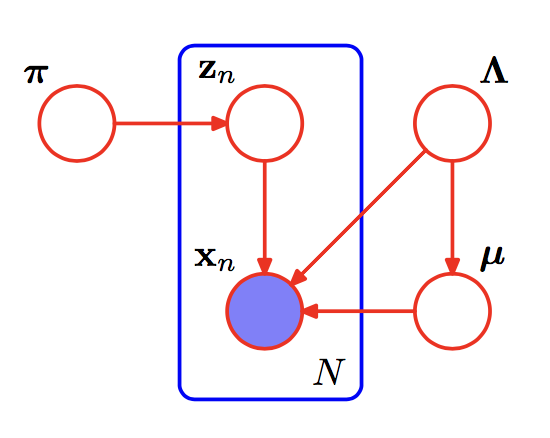
\includegraphics[width=8cm]{bayesian_gaussian_mixture.png}
    \end{center}
    \item \textbf{Variational Distribution} Joint distribution given by 
    \[
        p(\bX, \bZ, \bpi, \bmu, \bLambda) = 
        p(\bX | \bZ, \bmu, \bLambda) p(\bZ | \bpi) p(\bpi) p(\bmu | \bLambda) p(\bLambda)  
    \]
    We consider a variational distribution that factorizes between the latent variable and the parameters 
    \[
        q(\bZ, \bpi, \bmu, \bLambda) = q(\bZ) q(\bpi, \bmu, \bLambda)
    \]
    
\end{enumerate}




\href{2018_variational_inference_a_review_for_statisticians.pdf}{Variational Inference Review}

\begin{enumerate}
    \item \textbf{Idea} Posit a family of approximate densities $Q$ and find the member of that family $q^*$, parameterized by its variational parameters, that minimizes the Kullback-Leibler (KL) divergence to the exact posterior
    \[
        q^*(\bz) = \argmin_{q(\bz)\in Q} \kl{q(\bz)}{p(\bz | \bx)}
    \]
    \item \textbf{}
\end{enumerate}

 


\end{document}
 